\chapter{Appendix}

\section{Präsentation der grafischen Oberfläche der Berichtstools}

\begin{figure}[H]
    \centering
    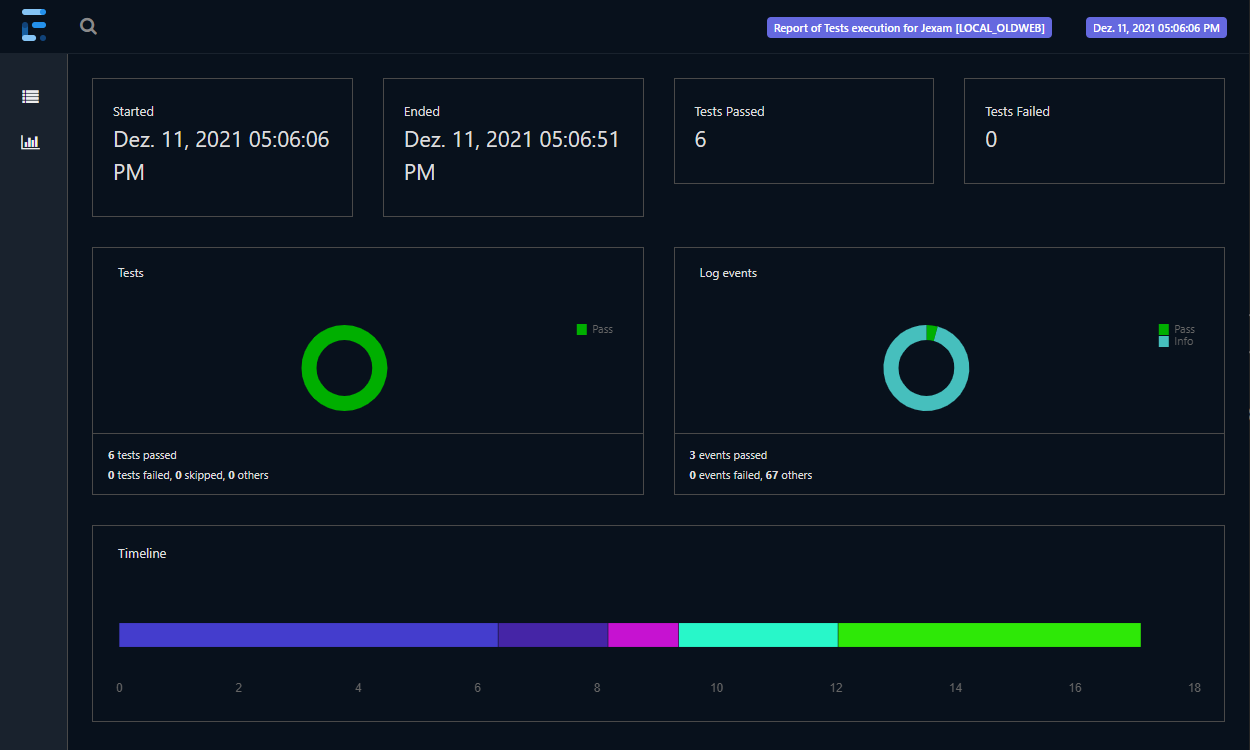
\includegraphics[scale=0.5]{images/extentReport2}
    \caption{Von Extent erstellter Bericht nach der Durchführung von UI-Tests} \label{fig:extent-report}
\end{figure}


\begin{figure}[H]
    \centering
    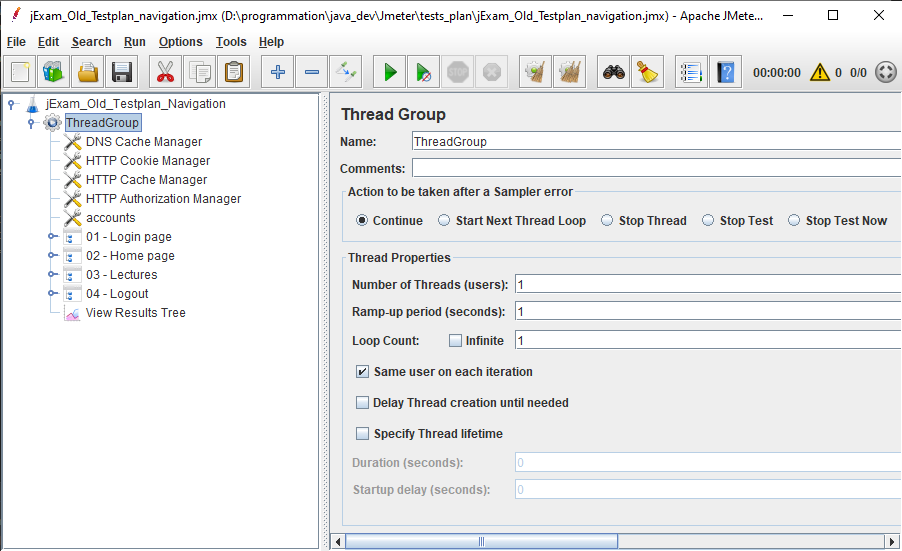
\includegraphics[scale=0.6]{images/jmeter-ui}
    \caption{Grafische Benutzeroberfläche von JMeter} \label{fig:jmeter}
\end{figure}

\begin{figure}[H]
    \centering
    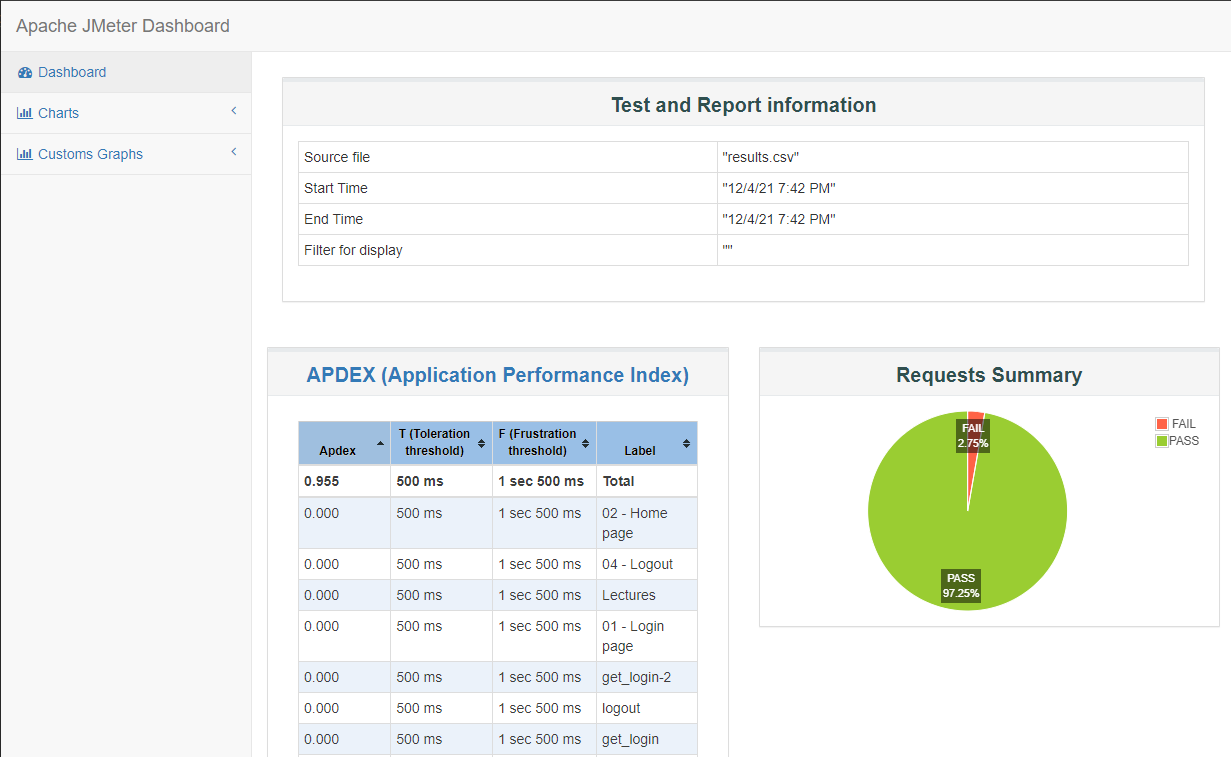
\includegraphics[scale=0.5]{images/jmeter-report}
    \caption{Vom JMeter-Skript erstellter Bericht nach der Durchführung der Tests} \label{fig:jmeter-report}
\end{figure}


\section{UML-Klassendiagramm und globale Struktur für einige Pakete der UI-Tests}

\begin{figure}[H]
    \centering
    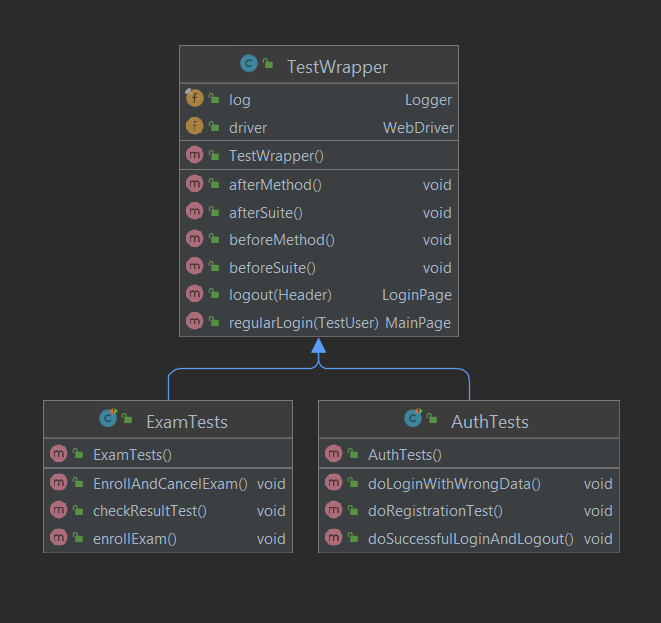
\includegraphics[scale=0.6]{images/system-test-uml}
    \caption{UML-Diagramm des Pakets systemTests} \label{fig:system-package}
\end{figure}

\begin{figure}[H]
    \centering
    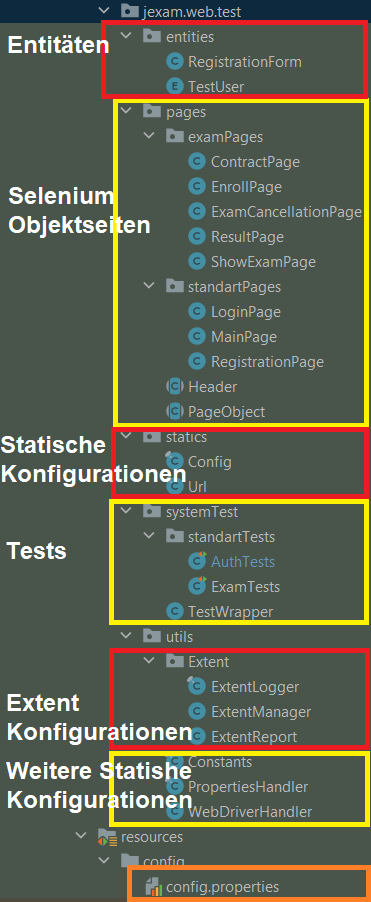
\includegraphics[scale=0.4]{images/ui-test}
    \caption{Genereller Struktur der UI-Tests} \label{fig:ui-test}
\end{figure}

\begin{figure}[H]
    \centering
    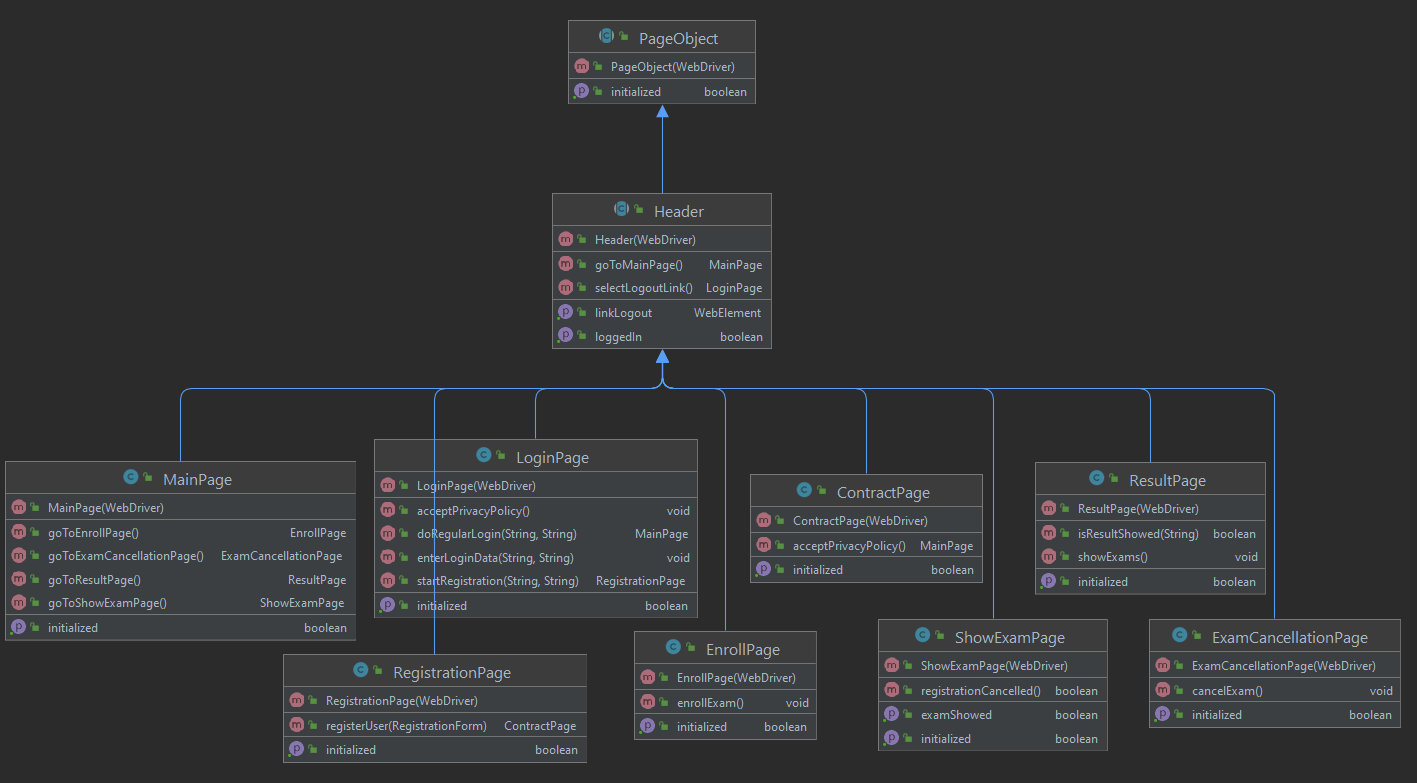
\includegraphics[scale=0.5]{images/pages_diagram}
    \caption{UML-Diagramm des Pakets pages} \label{fig:page-package}
\end{figure}

\section{Globale Struktur der Testinfrastruktur}

\begin{figure}[H]
    \centering
    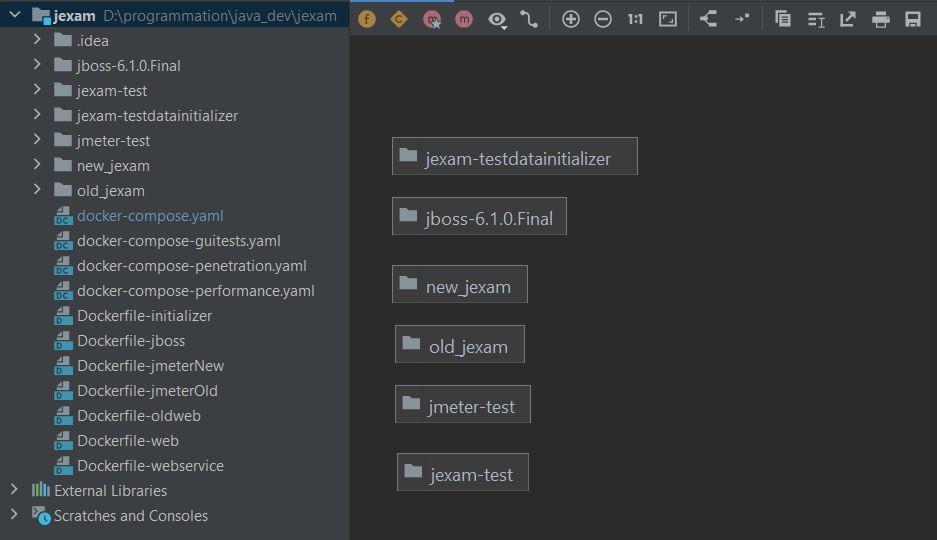
\includegraphics[scale=0.5]{images/global-structur}
    \caption{Globale Struktur der Testinfrastruktur} \label{fig:global-structur}
\end{figure}


\section{Einige Beispiele für Code Sources, die zum Verständnis beitragen}

\begin{lstlisting}[label={lst:docker-compose}, caption={Docker-Compose-Datei des Launcher-Dienstes}]

# Docker Compose File 
version: "3"

# docker network create jexam_network
# important command !
# docker-compose up
# docker-compose -f  docker-compose-penetration.yaml up
# docker-compose -f  docker-compose-performance.yaml up
# docker-compose -f  docker-compose-guitests.yaml up
# Must connect on TU Dresden vpn

services:

  jboss:
    build:
      context: ./
      dockerfile: ./Dockerfile-jboss
    container_name: jboss
    ports:
      - "1090:1090"
      - "1091:1091"
      - "1099:1099"
      - "40003:40003"
      - "4446:4446"
      - "4457:4457"
      - "4712:4712"
      - "4713:4713"
      - "4714:4714"
      - "9009:9009"

  oldweb:
    build:
      context: ./
      dockerfile: Dockerfile-oldweb
    container_name: oldweb
    stdin_open: true
    tty: true
    depends_on:
      - jboss
    ports:
      - "8085:8080"


  webservice:
    build:
      context: ./
      dockerfile: ./Dockerfile-webservice
    container_name: webservice
    stdin_open: true
    tty: true
    depends_on:
      - jboss
    ports:
      - "8081:8081"

  web:
    build:
      context: ./
      dockerfile: Dockerfile-web
    container_name: web
    stdin_open: true
    tty: true
    depends_on:
      - webservice
    ports:
      - "8080:8080"

  initializer:
    build:
      context: ./
      dockerfile: Dockerfile-initializer
    container_name: initializer
    stdin_open: true
    tty: true
    depends_on:
      - jboss
    volumes:
      - ./jexam-test/initializer-csv:/initializer/data/

networks:
  default:
    external:
      name: jexam_network
    
\end{lstlisting}


\begin{lstlisting}[label={lst:docker-file-web}, caption={Dockerfile Datei des jExam_New Container}]
# Dockerfile-Web (For jExam_New)

FROM openjdk:17-alpine
RUN apk --update add bash && apk --no-cache add dos2unix

COPY ./new_jexam/jexam-web /webapp

WORKDIR /webapp

# JARS kopieren

COPY ./new_jexam/jexam-webservice/. /webapp
COPY ./jboss-6.1.0.Final/server/jExamV5/lib/bos.jar /webapp
COPY ./jboss-6.1.0.Final/server/jExamV5/lib/common.jar /webapp
COPY ./jboss-6.1.0.Final/server/jExamV5/lib/csapis.jar /webapp

RUN rm -rf target
RUN rm -rf de.jexam.webservice

# CHANGE BASE_URL
RUN sed -i "s/localhost/webservice/g"  src/main/java/de/jexam/web/data/WebserviceConnector.java

RUN dos2unix mvnw

# RUN INSTALL JARS
RUN ./mvnw install:install-file -Dfile=bos.jar -DgroupId=de.jexam -DartifactId=bos -Dversion=1.0 -Dpackaging=jar
RUN ./mvnw install:install-file -Dfile=common.jar -DgroupId=de.jexam -DartifactId=common -Dversion=1.0 -Dpackaging=jar
RUN ./mvnw install:install-file -Dfile=csapis.jar -DgroupId=de.jexam -DartifactId=csapis -Dversion=1.0 -Dpackaging=jar

# INSTALL WEB CLASSES
RUN ./mvnw install:install-file -Dfile=/webapp/de.jexam.web.classes/target/classes-0.0.1-SNAPSHOT.jar -DgroupId=de.jexam -DartifactId=web-classes -Dversion=1.0 -Dpackaging=jar


RUN ./mvnw clean compile

ENTRYPOINT sleep 40;./mvnw spring-boot:run
\end{lstlisting}


